\chapter{Redes Neurais sem Peso}
    O cérebro humano faz parte do sistema nervoso e é considerado o núcleo de inteligência e aprendizado de um indivíduo. Composto por células nervosas chamadas de neurônios, permite atividades como o controle da ações motoras, integração dos estímulos sensoriais e atividades neurológicas como a memória e reconhecimento de padrões.
    
    As Redes Neurais Artificiais são baseadas em modelos matemáticos e técnicas computacionais inspiradas na estrutura neural dos organismos vivos. Geralmente são compostas por neurônios artificiais interconectados, que aplicam funções no sinal de entrada e alimentam a entrada do próximo neurônio formando uma rede, onde cada neurônio é responsável por parte do processamento da informação. Para cada conexão é atribuído um peso multiplicativo, que é um parâmetro a ser ajustado pelo algoritmo de otimização responsável pelo treinamento.
    
    As Redes Neurais sem Peso possuem neurônios que, ao invés de aplicar funções no sinal de entrada, participam do aprendizado de forma semelhante às memórias de acesso aleatório (RAM). A analogia biológica de tal neurônio é feita com o comportamento excitatório ou inibitório do sinal de entrada da árvore dendrítica. A "força" de um sinal de entrada da árvore dendrítica depende da altura que a conexão sináptica é posicionada, assim como as RAMs decodificam um sinal de entrada binário (excitatório/inibitório) em endereços de memória \cite{briefintrownn}.

    As redes neurais sem peso foram inspiradas no classificador \textit{n-tuples} \cite{bledsoe&browning}, que também aplica a decodificação do sinal de entrada para o reconhecimento de padrões. Uma grande aplicação para esse método é o reconhecimento de caracteres. Fotomosaicos com caracteres manuscritos eram representados através de fotocélulas, que por sua vez eram utilizadas como sinal de entrada binário, ou seja, cada fotocélula podia ser estar preenchida ou não formando um padrão binário que representa o caractere e é utilizado para o treinamento do modelo.
    
    A próxima seção explica detalhadamente o processo de codificação tal como descrito pelo parágrafo anterior e a arquitetura de Rede Neural sem Peso utilizada neste trabalho como ponto de partida para o entendimento do modelo de RNSP para previsão de séries temporais. 


\section{WiSARD}
    A arquitetura do modelo WiSARD (Wilkie, Stonhan and Aleksander Recognition Device) é composta por discriminadores, que são componentes responsáveis pela identidade de uma classe em um problema de classificação supervisionado. Cada discriminador é formado por um conjunto específico de memórias de acesso aleatório (RAMs), que são responsáveis por armazenar o padrão reconhecido no exemplo de entrada. A Figura~\ref{fig:wsd_disc} representa a estrutura da WiSARD seguida abaixo de um de seus Discriminadores.
    
    \begin{figure}[!ht] \label{fig:wsd_disc}
    \centering
    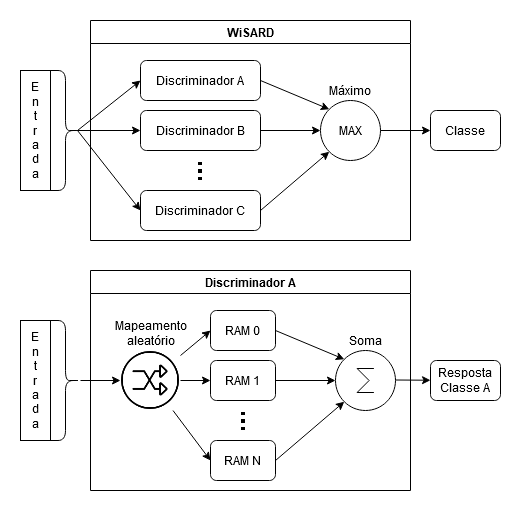
\includegraphics[width=5.0in]{img/wisard_discriminator.png}
    \caption{WiSARD e Discriminador. Em caso de empate, o operador máximo seleciona aleatoriamente um dos máximos encontrados.}
    \end{figure}
    
    O treinamento de um modelo WiSARD é dado pela escrita nas RAMs de cada discriminador, enquanto a classificação é dada pela leitura dessas posições de memória. A escrita se dá através de um mapeamento aleatório dos bits de entrada em um conjunto de endereços, que serão utilizados para apontar as posições de memória que devem ser escritas. Portanto, se faz necessária a utilização de uma entrada binária para a rede.
    
    \begin{figure}[!ht] \label{fig:wsd_train}
    \centering
    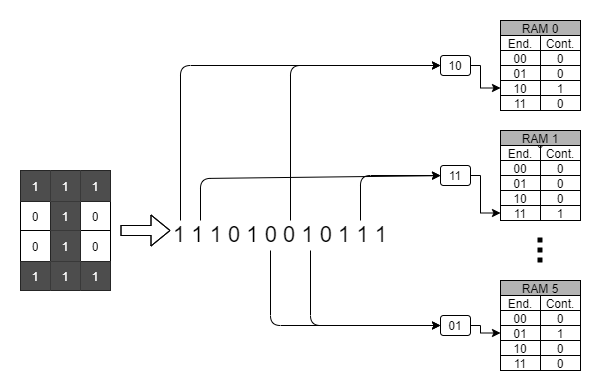
\includegraphics[width=5.0in]{img/wisard_training.png}
    \caption{Treinamento de um exemplo da classe I no seu respectivo discriminador.}
    \end{figure}
    
    A classificação é realizada lendo-se o conteúdo das RAMs de cada discriminador e comparando a entrada a ser classificada com o conteúdo das RAMs de cada discriminador a fim de descobrir à qual discriminador (ou classe) o exemplo pertence.
    
    \begin{figure}[!ht] \label{fig:wsd_classification}
    \centering
    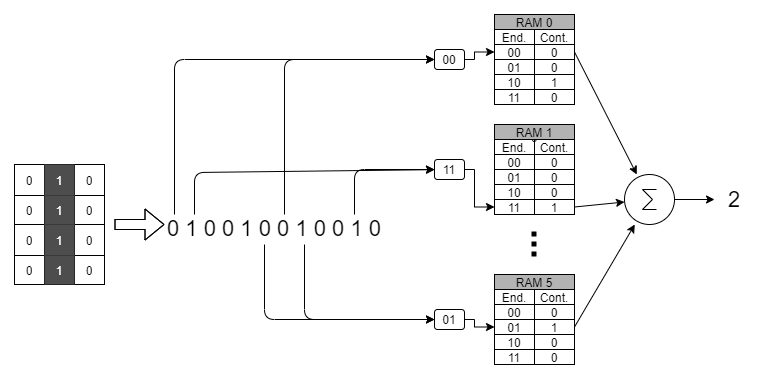
\includegraphics[width=5.0in]{img/wisard_classification.png}
    \caption{Classificação de um exemplo da classe I no seu respectivo discriminador já treinado.}
    \end{figure}
    
    Como o modelo requer uma entrada binária tanto para a etapa de treinamento quanto para a entrada de classificação, há uma dependência forte do pré-processamento dos dados a fim de obter uma representação razoável no formato binário, ou seja, transformar os dados de entrada em binário mantendo a capacidade de generalização do modelo. Algumas técnicas de pré-processamento serão apresentadas na Seção~\ref{sec:input_repr}.
    
    Um problema evidente no modelo WiSARD é a possibilidade de empate entre dois ou mais discriminadores, ou seja, mais de um discriminador com a mesma quantidade (máxima) de RAMs que acessaram posições escritas no momento da classificação. Portanto, para contornar tal problema, é utilizada a técnica \textit{bleaching}, introduzida em \cite{mentalimages} e primeiramente utilizada como \textit{bleaching} em \cite{advanceswns}. A técnica consiste em utilizar as posições de RAM como contadores ao invés de bits, e aplicar um valor limite na saída de cada RAM, de forma que a resposta do discriminador seja a soma do número de RAMs que apresentam o valor acessado superior ao valor limite escolhido como hiperparâmetro.

    \begin{figure}[!ht] \label{fig:bleaching}
    \centering
    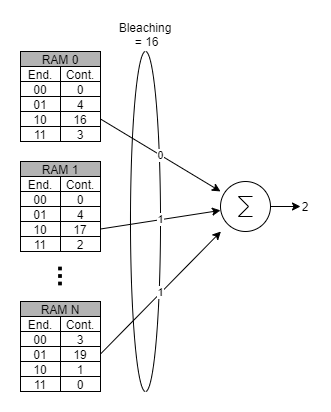
\includegraphics[width=3.0in]{img/bleaching.png}
    \caption{Exemplo de bleaching em um discriminador.}
    \end{figure}

\section{Regression WiSARD}
    A tarefa regressão, assim como a de classificação, é uma das tarefas mais abrangentes e divulgadas na área de aprendizado de máquina. Como descrito no capítulo anterior, o modelo WiSARD é utilizado para a resolução de problemas de classificação, mas, como alguns outros modelos de aprendizado de máquina, também pode ser utilizado para problemas de regressão, necessitando apenas de algumas modificações em sua arquitetura.
    A principal modificação necessária para utilização da WiSARD para a tarefa de regressão está na estrutura da RAM. Essa adaptação é um aumento de dimensionalidade dos valores armazenados em cada posição de memória, ou seja, enquanto na WiSARD cada posição de memória armazena um número inteiro (contador), na Regression WiSARD cada posição de memória armazena 2 valores: o número de acessos e o somatório do valor alvo dos exemplos que acessaram esta posição. A Figura~\ref{fig:ramxram} ilustra a diferença entre as duas arquiteturas.

    \begin{figure}[!ht] \label{fig:ramxram}
    \centering
    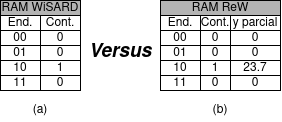
\includegraphics[width=4.0in]{img/ramxram.png}
    \caption{RAM da WiSARD na esquerda e RAM da Regression WiSARD na direita.}
    \end{figure}
    
    Para a etapa de treinamento essa é a única mudança necessária. Cada endereço, quando acessado, tem seu contador incrementado em 1 e seu valor incrementado do valor alvo do exemplo que acessou a posição. Já a etapa de inferência, após as RAMs já estiverem preenchidas, o acesso às posições continua sendo feito da mesma forma, porém a resposta do discriminador se torna uma função do contador e do valor das posições de memória acessadas.

    \begin{figure}[!ht] \label{fig:rew_discr}
    \centering
    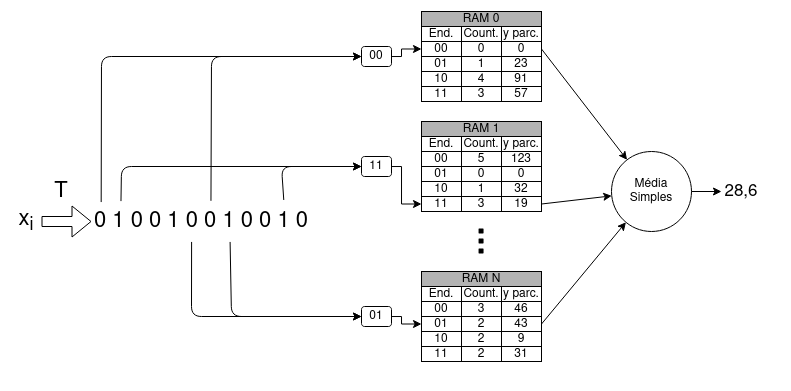
\includegraphics[width=6.0in]{img/rew_regression.png}
    \caption{Discriminador na etapa de inferência da Regression WiSARD transformando a entrada com a função T e agregando o valor de inferência com a função média simples.}
    \end{figure}

    O exemplo da Figura~\ref{fig:rew_discr} mostra o discriminador utilizando uma média simples como função dos valores da posição de memória acessada. É bem intuitivo e coerente pensar que essa função pode variar de acordo com o problema e ser tratada como um hiperparâmetro do modelo. Alguns exemplos de funções utilizadas são a média simples, mediana, média harmônica e média geométrica \cite{rew}.
    
    Além da função de agregação, é fato a permanência da necessidade de transformação da entrada para valores binários na Regression WiSARD. Para tal, existem diferentes técnicas de binarização que serão apresentadas na Seção~\ref{sec:input_repr}.

\section{Representação da entrada} \label{sec:input_repr}
    Tanto a WiSARD quanto a \textit{Regression} WiSARD possuem como requisito a representação binária da entrada. Como grande parte dos problemas do mundo real não são representados de forma binária, então é imprescindível a utilização de uma técnica de binarização que minimize a perda de informação para o modelo. Existem diversas técnicas já desenvolvidas que possuem vantagens e desvantagens quando utilizadas como preprocessamento para o treinamento de RNSPs, como o Limiar, a Transformação Termômetro, Filtro de \textit{Marr–Hildreth}, Filtro Laplaciano, entre outros. Um estudo comparativo de tais métodos pode ser encontrado em \cite{binenctec}.
    
    Para o escopo desse trabalho, será utilizada a transformação Termômetro, que possui as características necessárias para garantir um bom desempenho da rede. A transformação recebe 3 parâmetros: tamanho (\textit{sz}), valor mínimo (\textit{min}) e valor máximo (\textit{max}). O tamanho é a quantidade de bits que é utilizada para representar 1 número real, enquanto o valor mínimo e máximo representam o menor e o maior valor real possível assumido respectivamente. O algoritmo da transformação termômetro consiste na divisão do espaço entre o mínimo e o máximo em \textit{sz} pedações de mesmo tamanho, atribuindo um valor limite para cada uma das divisões. Em seguida, cada pedaço é preenchido por um bit 1 ou 0 dependendo se o valor que está sendo transformado está acima ou abaixo do valor limite. A Figura~\ref{fig:therm_ex} ilustra um número inteiro antes e após a transformação termômetro.
    
    \begin{figure}[!ht] \label{fig:therm_ex}
    \centering
    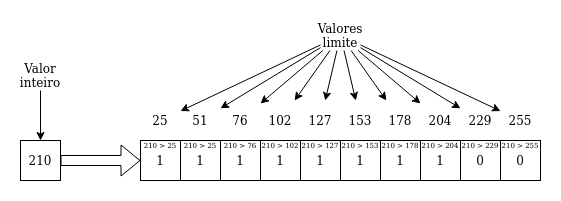
\includegraphics[width=6.0in]{img/therm_example.png}
    \caption{Transformação termômetro do número 210}
    \end{figure}

    É importante evidenciar que as técnicas utilizadas acima são fundamentais. A transformação dos números em binário modificando sua base de 10 para 2 tem um problema crucial. Ao mudar a base, os números perdem a propriedade de proximidade na representação, o que dificulta o processo de aprendizado da rede. Por exemplo, os números 11 e 12 possuem uma representação bem diferente quanto transformados da base 10 para 2, quando na verdade, deveriam ter representações próximas, pois são números próximos. A transformação termômetro garante essa propriedade. 
    
\section{Biblioteca wisardpkg}
    Quase todos os métodos descritos nas seções anteriores, incluindo as RNSPs WiSARD e Regression WiSARD, são implementados na biblioteca wisardpkg.

% Modelos implementados (WiSARD, Regression WiSARD)...

% Préprocessamentos implementados...
